\documentclass{article}
\usepackage{amsmath}
\usepackage{amsfonts}
\usepackage{amssymb}
\usepackage{graphicx}
\usepackage[parfill]{parskip}
\usepackage{matlab-prettifier}
\usepackage{listings}
\usepackage{xcolor}
\usepackage[a4paper, margin=2.54cm]{geometry}
\usepackage{float}

\title{MCEN 5228: Advanced Dynamics

HW1}
\author{David Akre}
\date{\today}

\begin{document}

\maketitle

\section{Consider the 2-3-1 Euler angle sequence that was used in the navigational computer for the Apollo Lunar Module (different than the 3-2-1 sequence shown in class). In this implementation, the 3-axis points out the front, the 2-axis out the right side, and the 1-axis along the vertical direction. Starting with a fixed frame $F = \{\hat{f}_x, \hat{f}_y, \hat{f}_z\}$, we first rotate an angle $\theta$ about the 2-axis to generate the intermediate frame $I_1 = \{\hat{x}', \hat{y}', \hat{z}'\}$, then an angle $\psi$ about the 3-axis to generate the intermediate frame $I_2 = \{\hat{x}'', \hat{y}'', \hat{z}''\}$, and finally an angle $\phi$ about the 1-axis to generate the final orientation of the body frame $B = \{\hat{e}_x, \hat{e}_y, \hat{e}_z\}$, as shown in the figure.}

As noted in lecture and in Goldstein pg 143, positive CCW rotations about a single axis results in a passive transformations of the frame of reference. This is what I'll be using for all the parts in the homework unless specified otherwise.

\subsection{As was done in class for the 3-2-1 sequence, construct a 3D diagram for the 2-3-1 sequence as described above showing the three successive rotations, all intermediate coordinate frames, and the three Euler rate vectors. Be sure to trace out the tip displacements of the unit vectors with a dashed line, and start with a fixed frame that has a similar orientation to the frame shown in that figure.}

Below are screenshots taken of a matlab script I wrote which performs the 2-3-1 Euler angle rotations based on the coordinate system in the problem statement. The fainter vector depicts the vector in the previous frame, the bolder vector in the same color depicts the vector in the newly rotated frame (i.e., intermediate), and the dashed arrow indicates the direction of rotation from previous to new based on the tip displacement. I have the matlab script attached to this document for reference as well as all 2-3-1 rotations in one plot (apologies for it being smaller but I think you can zoom in to see it better).

The euler rate vector is aligned with the coordinate vector being rotated which I will identify in each step which direction its in.

\newpage
First rotation about the 2-axis (green vector) and the euler rate vector is aligned directly to this green vector points towards us.
\begin{figure}[H]
    \centering
    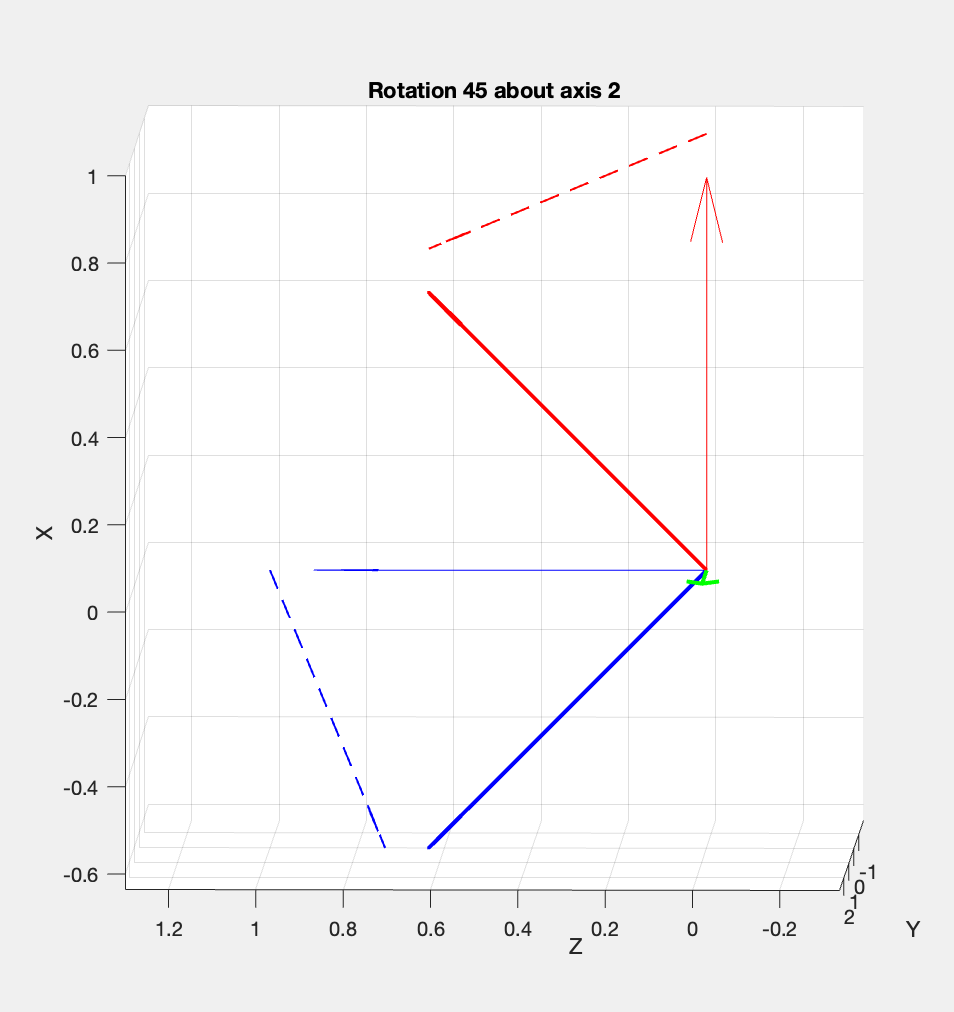
\includegraphics[width=0.8\linewidth]{2_axis_rotation.png}
    \caption{2-axis Rotation}
\end{figure}

\newpage
Second rotation about the 3-axis (blue vector) and the euler rate vector is aligned directly to the blue vector pointing towards us.
\begin{figure}[H]
    \centering
    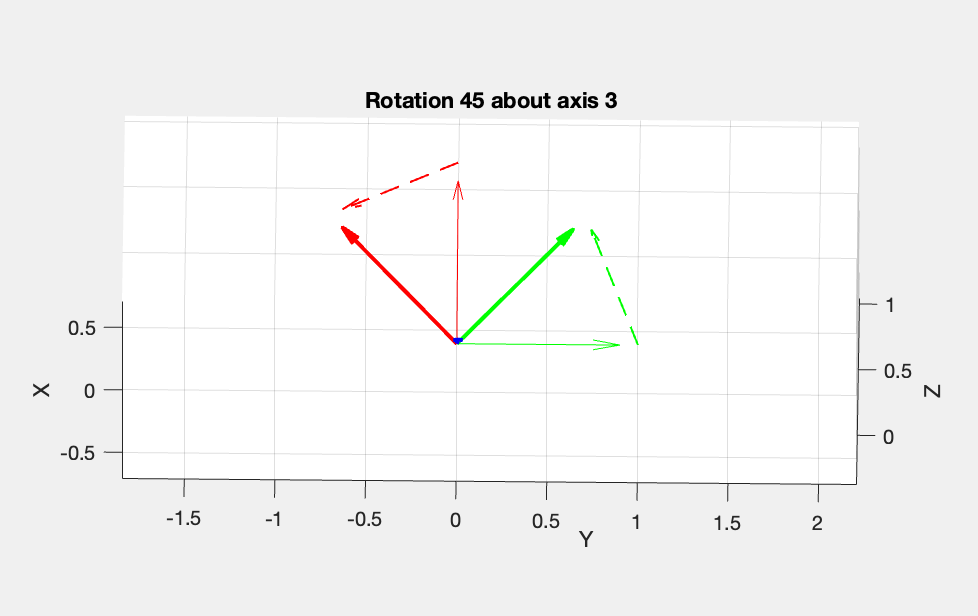
\includegraphics[width=0.8\linewidth]{3_axis_rotation.png}
    \caption{3-axis Rotation}
\end{figure}

Third rotation about the 1-axis (red vector) and the euler rate vector is aligned directly to this red vector pointing towards us.
\begin{figure}[H]
    \centering
    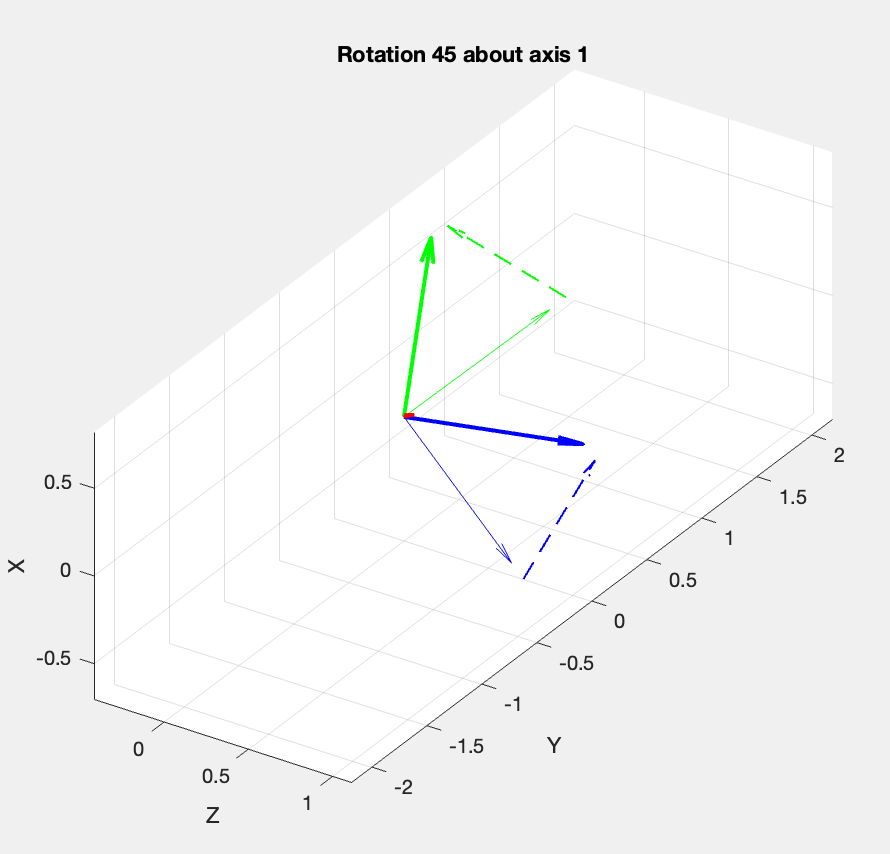
\includegraphics[width=0.8\linewidth]{1_axis_rotation.png}
    \caption{1-axis Rotation}
\end{figure}

All rotations from matlab with common perspective view point:
\begin{figure}[H]
    \centering
    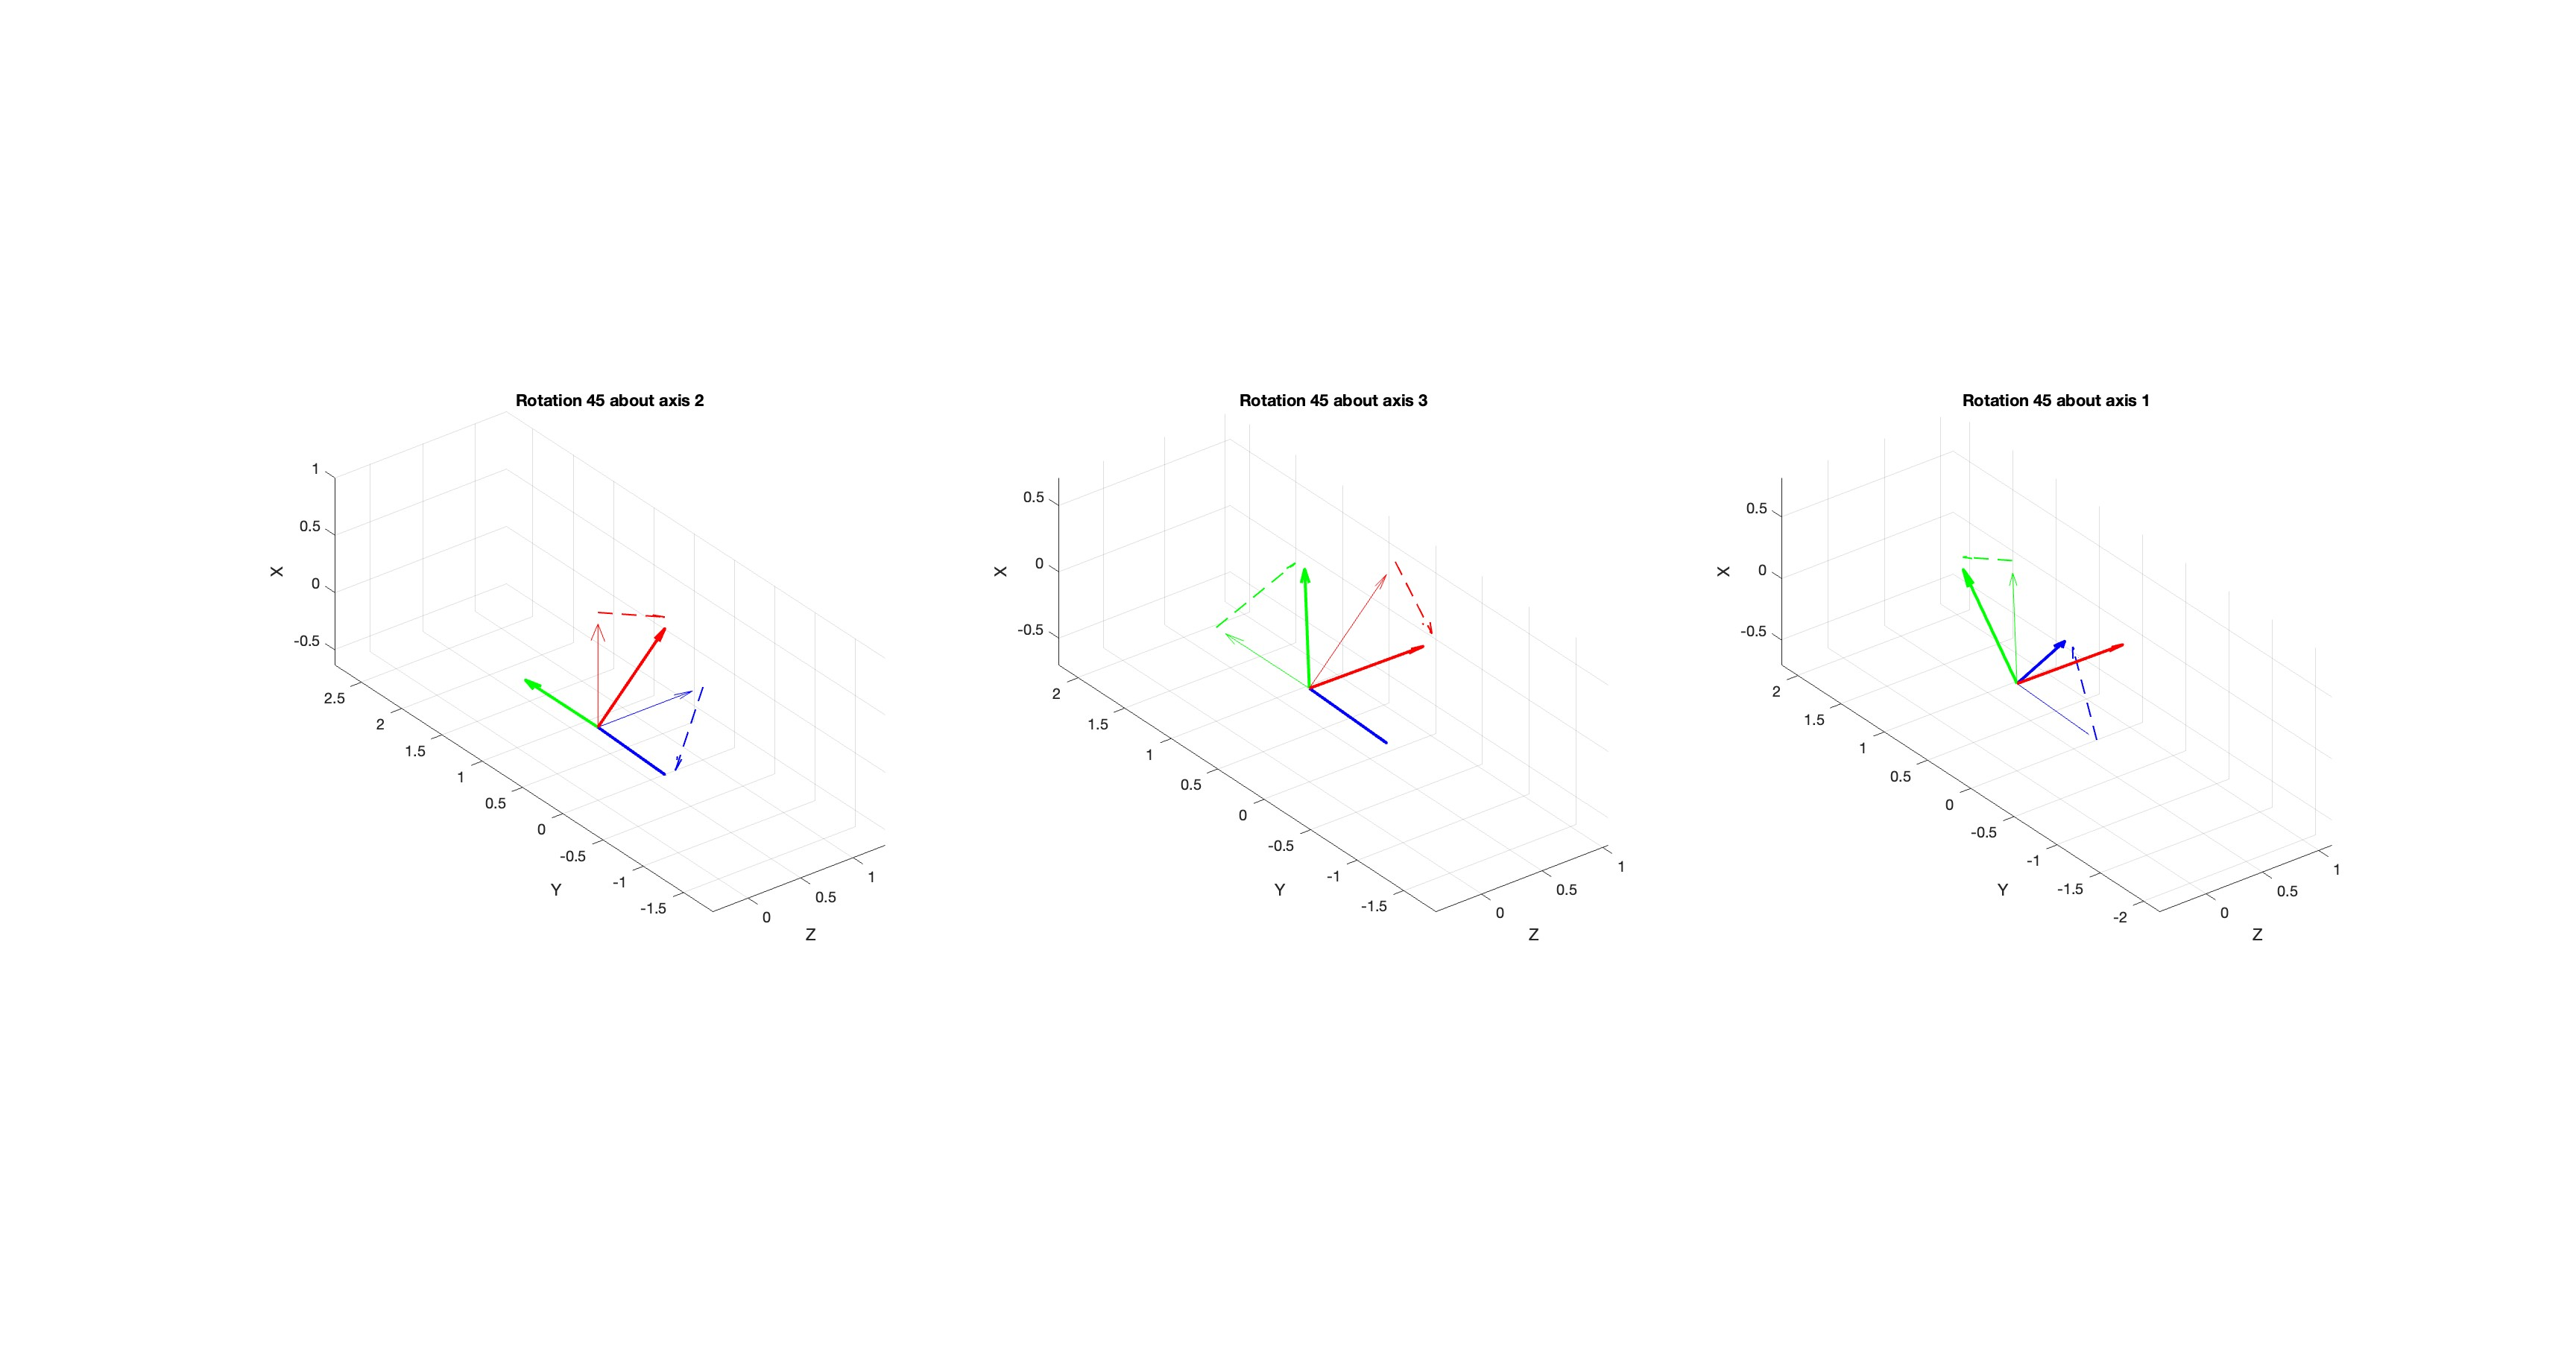
\includegraphics[width=\linewidth]{2_3_1_rotations.jpg}
    \caption{2-3-1 axis Rotations}
\end{figure}

Matlab script for reference (note coordinate frame is aligned to the problem before rotation sequence is applied).
\lstinputlisting[frame=single, numbers=left, style=Matlab-editor]{rotate_frame.m}

\subsection{Find the three rotation matrices $R_2(\theta)$, $R_3(\psi)$, and $R_1(\phi)$ which define the sequence of rotations from the fixed frame $F$ to the body frame $B$, and compute the transformation matrix $R_{BF}(\theta, \phi, \psi)$ that maps coordinates from the frame F to B for this Euler angle sequence.}

Applying the first rotation matrix $R_2(\theta)$ from $F \to I'$ can be described as: 

\begin{align*}
    & R_2(\theta) = \begin{bmatrix}\cos(\theta) & 0 & -\sin(\theta) \\ 0 & 1 & 0 \\ \sin(\theta) & 0 & \cos(\theta)\end{bmatrix} \\
    & R_{F \to I'} = R_2(\theta)
\end{align*}

Next applying the second rotation matrix $R_3(\psi)$ from $I' \to I''$ can be described as: 

\begin{align*}
    & R_3(\psi) = \begin{bmatrix}\cos(\psi) & \sin(\psi) & 0 \\ -\sin(\psi) & \cos(\psi) & 0 \\ 0 & 0 & 1\end{bmatrix} \\
    & R_{I' \to I''} = R_3(\psi) R_2(\theta) = \begin{bmatrix} \cos(\psi) \cos(\theta) & \sin(\psi) & -\cos(\psi) \sin(\theta) \\ -\sin(\psi) \cos(\theta) & \cos(\psi) & \sin(\psi) \sin(\theta) \\ \sin(\theta) & 0 & \cos(\theta)\end{bmatrix}
\end{align*}

The last rotation matrix $R_1(\phi)$ from $I'' \to B$ can be described as: 

\begin{align*}
    & R_1(\phi) = \begin{bmatrix}1 & 0 & 0\\ 0 & \cos(\phi) & \sin(\phi) \\ 0 & -\sin(\phi) & \cos(\phi)\end{bmatrix} \\
    & R_{I'' \to B} = R_1(\phi) R_{I' \to I''} \\
    & R_{BF} = \begin{bmatrix} \cos(\psi) \cos(\theta) & \sin(\psi) & -\cos(\psi) \sin(\theta) \\ -\cos(\phi) \sin(\psi) \cos(\theta) + \sin(\phi) \sin(\theta) & \cos(\phi) \cos(\psi) & \cos(\phi) \sin(\psi) \sin(\theta) + \sin(\phi) \cos(\theta) \\ \sin(\phi) \sin(\psi) \cos(\theta) + \cos(\phi) \sin(\theta) & -\sin(\phi) \cos(\psi) & -\sin(\phi) \sin(\psi) \sin(\theta) + \cos(\phi) \cos(\theta)\end{bmatrix}
\end{align*}

$R_{BF}$ is shown above as the mapping from frame $F$ to $B$. Also note that in the above matlab script (i.e., lines 6-16) shows the coordinates being transformed by the 2-3-1 Euler angles step-by-step.

\subsection{Derive the transformation between the body frame yaw, pitch, and roll rates $\omega^{F \to B} = ( p, q, r )^T$ and the heading, attitude, and bank angle rates $\dot{\Theta} = (\dot{\phi}, \dot{\theta}, \dot{\psi})^T$ (that is, find the equivalent of the $E(\Theta )$ matrix in the equation $\dot{\Theta} \omega^{F \to B}$ for this sequence of Euler angles). Hint: $A^{-1} = adj(A) / det(A)$ where $adj(A)$ is the adjoint of $A$.}

For our 2-3-1 axis rotation we can derive the transformation between the body frame rates and angle rates in the following manner:
\begin{align*}
    & [\omega^{F \to B}]_B = \begin{bmatrix} p \\ q \\ r \end{bmatrix} = \begin{bmatrix} \dot{\phi} \\ 0 \\ 0 \end{bmatrix} + R_{BI''} \begin{bmatrix} 0 \\ 0 \\ \dot{\psi} \end{bmatrix} + R_{BI'} \begin{bmatrix} 0 \\ \dot{\theta} \\ 0 \end{bmatrix} \\
    & = \begin{bmatrix} \dot{\phi} \\ 0 \\ 0 \end{bmatrix} + \begin{bmatrix} 1 & 0 & 0 \\ 0 & \cos{\phi} & \sin(\phi) \\ 0 & -\sin(\phi) & \cos(\phi) \end{bmatrix} \begin{bmatrix} 0 \\ 0 \\ \psi \end{bmatrix} + \begin{bmatrix}\cos(\psi) & \sin(\psi) & 0 \\ -\cos(\phi) \sin(\psi) & \cos(\phi) \cos(\psi) & \sin(\phi) \\ \sin(\phi) \sin(\psi) & -\sin(\phi) \cos(\psi) & \cos(\phi)\end{bmatrix} \begin{bmatrix} 0 \\ \dot{\theta} \\ 0 \end{bmatrix} \\
    & p = \dot{\phi} + \dot{\theta}\sin(\psi) \\
    & q = \dot{\psi}\sin(\psi) + \cos{\phi}\cos(\psi) \dot{\theta} \\
    & r = \dot{\psi}\cos(\phi) - \sin{\phi}\cos(\psi) \dot{\theta}
\end{align*}
Thus the mapping to $[\omega^{F \to B}]_B$ is:
\begin{align*}
    & \begin{bmatrix}p \\ q \\ r\end{bmatrix} = \begin{bmatrix} 1 & \sin(\psi) & 0 \\ 0 & \cos(\phi) \cos(\psi) & \sin(\phi) \\ 0 & -\sin(\phi) \cos(\psi) & \cos(\phi) \end{bmatrix} \begin{bmatrix} \dot{\phi} \\ \dot{\theta} \\ \dot{\psi}\end{bmatrix}
\end{align*}
Now to go from $[\omega^{F \to B}]_B$ to $\dot{\Theta}$ we need to invert the above mapping which introduces a singularity which will be identified in the below section. This new mapping is called $E(\Theta)$. To invert the mapping above we need to take the adjoint and divide it by the determinant. So let $M$ be our mapping described above and to get to $E(\Theta)$ we need to invert $M^{-1}$.

The determinant calculation:
\begin{align*}
    & \det(M) = \cos(\psi)
\end{align*}
The adjoint calculation:
\begin{align*}
    & adj(M) = \text{Matrix of cofactors } C_{i,j} \text{ described below} \\
    & C_{0,0} = \cos(\psi) \\
    & C_{0,1} = 0 \\
    & C_{0,2} = 0 \\
    & C_{1,0} = -\sin(\psi) \cos(\phi) \\
    & C_{1,1} = -\cos(\phi) \\
    & C_{1,2} = \sin(\phi) \cos(\psi) \\
    & C_{2,0} = \sin(\psi) \sin(\phi) \\
    & C_{2,1} = \sin{\phi} \\
    & C_{2,2} = -\cos{\phi} \cos{\psi}
\end{align*}
Altogether we arive at the inverse and mapping $E(\Theta)$:
\begin{align*}
    & E(\Theta) = \frac{1}{\cos(\psi)} \begin{bmatrix} \cos(\psi) & 0 & 0 \\ -\sin(\psi) \cos(\phi) & -\cos(\phi) & \sin(\phi) \cos(\psi) \\ \sin(\psi) \sin(\phi) & \sin(\phi) & -\cos(\phi) \cos(\psi)\end{bmatrix} \\
    & E(\Theta) = \begin{bmatrix} 1 & 0 & 0 \\ -\tan(\psi) \cos(\phi) & -\frac{\cos(\phi)}{\cos(\psi)} & \sin(\phi) \\ \tan(\psi) \sin(\phi) & \frac{\sin(\phi)}{\cos(\psi)} & -\cos(\phi) \end{bmatrix}
\end{align*}

\subsection{For which physical orientations does this transformation become singular?}

From the above determinant calculation (i.e., $\cos(\psi)$) we can see physical orientations of $\psi = \overset{+}{\underset{-}{\phantom{=}}}[\frac{\pi}{2}, \frac{3*\pi}{2}, ...]$ will make the above transformation singular.

\section{In lecture the relationship between the Euler rates and the body rates for the 3-2-1 Euler angle sequence was shown to be \\
$\begin{bmatrix}p \\ q \\ r\end{bmatrix} = \begin{bmatrix}1 & 0 & -\sin(\theta) \\ 0 & \cos(\phi) & \sin(\phi) \cos(\theta) \\ 0 & -\sin(\phi) & \cos(\phi) \cos(\theta) \end{bmatrix} \begin{bmatrix}\dot{\phi} \\ \dot{\theta} \\ \dot{\psi} \end{bmatrix}$ \\
As was done for the first of the three equations in class, use geometry (not rotation matrices) to derive the second two equations. You will need to think about 2-D cross sections of the 3-D rotation diagram in order to obtain the correct projections of the Euler rate vectors in the body axes.}

First looking at the plane spanned by $\dot{\psi}$ and $\dot{\phi}$ to deteremine $p$.

\begin{figure}[H]
    \centering
    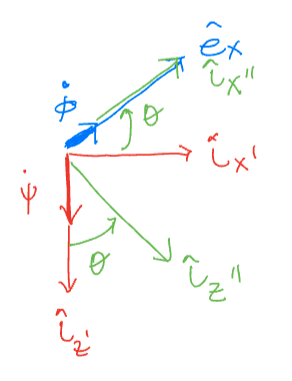
\includegraphics[width=0.8\linewidth]{plane_spanned_by_psi_phi.png}
    \caption{Plane Spanned by $\dot{\psi}$ \& $\dot{\phi}$ in class}
\end{figure}

Direction cosines calculations:
\begin{align*}
    & p = <\dot{\psi}, \hat{e}_x> + <\dot{\theta}, \hat{e}_x> + <\dot{\phi}, \hat{e}_x> \\
    & <\dot{\theta}, \hat{e}_x> = 0 \\
    & <\dot{\psi}, \hat{e}_x> = \dot{\psi} \sin(\theta) \\
    & <\dot{\phi}, \hat{e}_x> = \dot{\phi} \\
    & p = -\dot{\psi} \sin(\theta) + \dot{\phi}
\end{align*}

The next plane to look at is the one spanned by $\dot{\theta}$ and $\dot{\psi}$ in the interim rotation frame.

\begin{figure}[H]
    \centering
    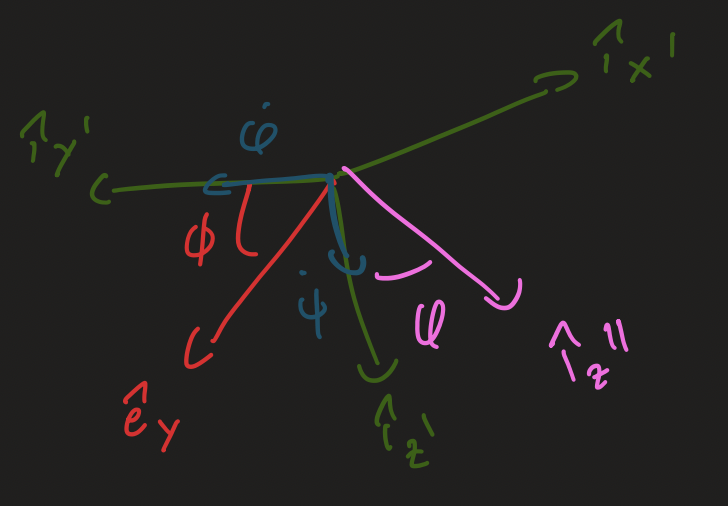
\includegraphics[width=0.8\linewidth]{plane_spanned_by_theta_psi.png}
    \caption{Plane Spanned by $\dot{\theta}$ \& $\dot{\psi}$}
\end{figure}

Direction cosines calculations:
\begin{align*}
    & q = <\dot{\psi}, \hat{i}_y'> + <\dot{\theta}, \hat{i}_y'> + <\dot{\phi}, \hat{i}_y'> \\
    & <\dot{\psi}, \hat{i}_y'> = \dot{\psi}[\cos(\phi)[\cos(\theta) + \sin(\theta)] + \sin(\phi)[\cos(\theta) + \sin(\theta)]] \\
    & = \dot{\psi}[0 + 0 + \sin(\phi)\cos(\theta) + 0] \text{ where } \sin(\phi = \frac{\pi}{2}) = 1 \text{ and } \cos(\theta = 0) = 1 \implies \dot{\psi} \\
    & <\dot{\theta}, \hat{i}_y'> = \dot{\theta} \cos(\phi) + \dot{\theta} \sin(\phi) \\
    & = \dot{\theta} \cos(\phi) \text{ where } \phi = 0 \implies \dot{\theta} \\
    & <\dot{\phi}, \hat{i}_y'> = 0 \\
    & q = \dot{\theta} \cos{\phi} + \dot{\psi} \sin(\phi)\cos{\theta}
\end{align*}

Using the same plane defined above we have $\dot{\psi}$ as one of the spanning vectors which we can use define $r$. Thus the following direction cosines calculation are:
\begin{align*}
    & r = <\dot{\psi}, \hat{i}_z'> + \dot{\theta}, \hat{i}_z'> + <\dot{\phi}, \hat{i}_z'> \\
    & <\dot{\psi}, \hat{i}_z'> = \dot{\psi}[\cos(\phi)[\cos(\theta) + \sin(\theta)] + \sin(\phi)[\cos(\theta) + \sin(\theta)]] \\
    & = \dot{\psi}[\cos(\phi) \cos(\theta) + 0 + 0 + 0] \text{ since this is the first rotation } \phi = 0, \theta = 0 \implies \cos(\phi) \cos(\theta) = 1 \\
    & <\dot{\theta}, \hat{i}_z'> = \dot{\theta} \cos(\phi) + \dot{\theta} \sin(\phi) \\
    & = - \dot{\theta} \sin(\phi) \text{ where pitch rate is in the direction of the yaw rate when the frame has (-)sin roll component } \\
    & <\dot{\phi}, \hat{i}_z'> = 0 \\
    & r = \dot{\psi} \cos(\phi) \cos(\theta) - \dot{\theta} \sin(\phi)
\end{align*}

The $\begin{bmatrix} p & q & r\end{bmatrix}^T$ is now aligned with the 3-2-1 rotation matrix based on the geometric intuition and direction cosines method.

\end{document}